\section{Background on sparse GGM}

\begin{frame}
  \frametitle{\alert{Gaussian} Graphical Model}

  Suppose   the   profiles   of    the   genes/OTUs   is   such   that
  $\mathbf{X}_i\sim\mathcal{N}(\bzr_p,\invcov^{-1})$.

  \begin{itemize}
  \item independence is equivalent to null covariance/correlation
  \item  \alert{  conditional  independence is  equivalent  to  null
      partial covariance/correlation}
    \begin{equation*}
      \label{eq:parcor2invcov}
      \rho_{ij}      =  -\invcov_{ij}      /
      \sqrt{\invcov_{ii} \invcov_{jj}}, \qquad \invcov_{ii}=
      \var(X_i|X_{\backslash \{i,j\}})^{-1}
    \end{equation*}
  \end{itemize}

  
  \begin{block}{Conditional independence structure}
    \vspace{-.5cm}
    \begin{equation*}
      (i,j)  \notin  \mathcal{E}  \Leftrightarrow  Y_i  \indep  Y_j  |
      Y_{\backslash \{i,j\}} \Leftrightarrow \invcov_{ij} = 0.
    \end{equation*}
  \end{block}
  
  \vspace{-.5cm}
  \begin{block}{Graphical interpretation}
    \vspace{-.5cm}
    \begin{center}
      \begin{tabular}{c@{\hspace{2cm}}c}
        \begin{tabular}{c}
          \small $\mathcal{G}=(\mathcal{P},\mathcal{E})$ \\
          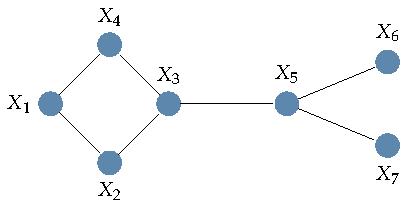
\includegraphics[width=.3\textwidth]{graph}
        \end{tabular}
     &
       \begin{tabular}{c}
         \small $\invcov$\\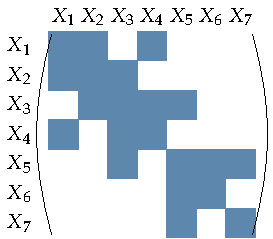
\includegraphics[width=.2\textwidth]{Markovadjacency}
       \end{tabular}
      \end{tabular}
    \end{center}
  \end{block}
  \vspace{-.5cm}
  
  \rsa Network reconstruction is (roughly) a variable selection problem
\end{frame}

\begin{frame}
  \frametitle{Gaussian Graphical Model and Linear Regression}

  \begin{block}{Linear regression viewpoint}
    Gene expression $X_j$ is linearly explained by the other genes':

    \begin{equation*}
      \bX_j | \bX_{ \setminus j} = - \sum_{k \neq j}
      \frac{\invcov_{jk}}{\invcov_{jj}} \bX_{k} + \varepsilon_j,\quad \varepsilon_j
      \sim \mathcal{N}(0,\invcov_{jj}^{-1}), \quad \varepsilon_j \perp X_j
      \end{equation*}
      Conditional  on its  neighborhood,  other profiles  do not  give additional insights
    \begin{equation*}
      \bX_j | \bX_{ \setminus j} =
       \sum_{k \in \text{ne(j)}} \beta_{jk} \bX_k + \varepsilon_j
      \quad         \text{with         }         \beta_{jk}         =
      -\frac{\Theta_{jk}}{\Theta_{jj}}.
    \end{equation*}
  \end{block}

  % \vspace{-.5cm}
  % \begin{overlayarea}{\textwidth}{.45\textheight}
  %   \begin{block}{Graphical Interpretation}
  %     \vspace{-.5cm}
  %     \begin{center}
  %       \begin{scriptsize}
  %         \begin{tabular}{cc}
  %           Local Markov property & Global Markov property \\
  %           conditioning on the neighborhood & conditioning on a separating node\\
  %           \includegraphics[width=.4\textwidth]{localMarkov}
  %           & \includegraphics[width=.4\textwidth]{globalMarkov}\\
  %         \end{tabular}
  %       \end{scriptsize}
  %     \end{center}
  %   \end{block}
  % \end{overlayarea}

  \vfill
  \alert{$\rightsquigarrow$ ``Neighborhood'' selection}

\end{frame}

\begin{frame}
  \frametitle{Gold standard penalized approaches (1)}
  \framesubtitle{Use $\ell_1$ for both regularizing and promoting \textit{sparsity}}

  \begin{overlayarea}{\textwidth}{\textheight}

    \begin{block}{Penalized   likelihood  (Banerjee   \textit{et
          al.}, Yuan and Lin, 2008)}
      \vspace{-1em}
\begin{equation*}
  \label{eq:MLE_l1}
  \widehat{\invcov}^{\text{glasso}}_\lambda = \arg \max_{\invcov \in \mathcal{S}^+_p} \; \log
  \det(\invcov) - \trace{\invcov \empcov} -
  \lambda\ \|\invcov\|_{\ell_1}.
\end{equation*}
    \end{block}
    \vspace*{-1.5em}
    
    \begin{itemize}
    \item[\textcolor{green}{$+$}] symmetric, positive-definite
    \item[\textcolor{red}{$-$}]       solved      by       the
      ``Graphical-Lasso''                 ($\mathcal{O}(p^3)$,
      \textit{Friedman et al, 2007}).
    \item \texttt{R}-packages \textbf{glasso}, \textbf{quic}, \textbf{huge}.
    \end{itemize}
    
    \vfill
    
    \begin{block}{Neighborhood    Selection   (Meinshausen    \&
        B\"ulhman, 2006)}<2-> \vspace*{-1em}
\begin{equation*}
  \label{eq:MB_pseudo}
  \hat\bB^{\text{ns}}  = \argmin_{\bB\in\Rset^{p\times  p}, \diag(\bB)
    =    \bzr_p}    \frac{1}{2}    \trace{\bB^\top\empcov    \bB}    -
  \trace{\bB^\top\empcov} + \lambda \|\bB\|_{\ell_1}.
\end{equation*}
      \vspace*{-1.5em}
    \end{block}
    
    \onslide<2>{
      \begin{itemize}
      \item[\textcolor{red}{$-$}]     not     symmetric,     not
        positive-definite
      \item[\textcolor{green}{$+$}]   $p$   Lasso  solved   with
        Lars-like   algorithms   ($\mathcal{O}(npd)$   for   $d$
        neighbors).
      \item \texttt{R}-package \textbf{huge}.
      \end{itemize}
    }
     
\end{overlayarea}      

\end{frame}

\begin{frame}
  \frametitle{Gold standard penalized approaches (2)}
  \framesubtitle{Use $\ell_1$ for both regularizing and promoting \textit{sparsity}}

  \begin{overlayarea}{\textwidth}{\textheight}
        
    \begin{block}{CLIME -- Pseudo-likelihood  (Cai et al., 2011;
        Yuan, 2010)}<1->
      \vspace*{-1.5em}
      \begin{equation*}
        \widehat{\invcov}^{\text{clime}}_\lambda  = \argmin_{\invcov}
        \left\|   \invcov \right\|_1 \text{ subjected to }
        \left\|   \empcov \invcov - \mathbf{I} \right\|_\infty\leq \lambda
      \end{equation*}
      \vspace*{-1.5em}
    \end{block}
    
    \begin{itemize}
    \item[\textcolor{red}{$-$}] not positive-definite
    \item[\textcolor{green}{$+$}]  $p$ linear  programs easily
      distributed ($\mathcal{O}(p^2d)$ for $d$ neighbors).
    \item \texttt{R}-package \textbf{fastclime} (dedictated imp. up to p=6!).
    \end{itemize}

      \vspace*{-.5em}
    
    \begin{block}{Sparse PArtial  Correlation Estimation (SPACE)
        (Peng 2009; Khare 2014 )}<2-> 
      \vspace*{-2em}
      \begin{equation*}
        \left(\widehat{\boldsymbol\rho}_\lambda^{\text{space}}, \mathrm{diag}({\boldsymbol\Theta})\right) =
        \argmin_{\boldsymbol\rho,\mathrm{diag}({\boldsymbol\Theta})} \frac{1}{2}
        \sum_{j=1}^p \omega_j \left\|
          \bX_j - \sum_{k=1}^p \rho_{jk} \sqrt{\frac{{\invcov}_{kk}}{{\invcov}_{jj}}}
          \bX_k \right\|_{\ell_2}^2 + \lambda\ \| \boldsymbol\rho \|_{\ell_1}
      \end{equation*}
      \vspace*{-1.5em}
    \end{block}
    
    \onslide<2>{
      \begin{itemize}
      \item[\textcolor{green}{$+$}]  for  fixed variances,  same
        cost as neighborhood selection.
      \item[\textcolor{red}{$-$}]    alternate    procedure    without
        guarantees on the number of iterates
      \item \texttt{R}-package \textbf{gconcord}.
      \end{itemize}
    }
      
\end{overlayarea}      

\end{frame}

\begin{frame}
  \frametitle{Practical implications of theoretical results}

  \begin{block}{Selection    consistency    (Ravikumar,    Wainwright,
      2009-2012)}<1->                                           Denote
    $d=\max_{j\in\mathcal{P}}(\mathrm{degree_j})$.  Consistency for an
    appropriate $\lambda$ and
    \begin{itemize}
    \item  $n\approx\mathcal{O}(d^2\log(p))$ for  the graphical  Lasso
      and Clime.
    \item $n\approx\mathcal{O}(d\log(p))$  for   neighborhood
      selection (sharp).
    \end{itemize}
    \textit{(Irrepresentability) conditions are not strictly
    comparable\dots}
  \end{block}

  \vfill

  \begin{block}{Ultra high-dimension phenomenon (Verzelen,  2011)}
    Minimax risk for sparse regression with $d$-sparse models: useless
    when
    \begin{equation*}
    \frac{d \log(p/d)}{n} \geq 1/2, \qquad (\mathrm{e.g.}, n=50, p=200, d\geq 8).
    \end{equation*}
    \textit{Good news! when $n$ is small, we don't need to solve
      huge problems because they can't but fail.}
  \end{block}

\end{frame}

\begin{frame}
  \frametitle{Model selection}
  
  \begin{block}{Cross-validation}
    Optimal in terms of \alert{prediction}, not in terms of selection
  \end{block}

  \begin{block}{Information based criteria}
    \begin{itemize}
    \item GGMSelect (Girault \textit{et al}, '12) selects among a family of candidates.
    \item Adapt IC to sparse high dimensional problems, e.g.
    \begin{equation*}
      \text{EBIC}_\gamma(\widehat{{\boldsymbol\Theta}}_\lambda)  =   -2 \textrm{loglik}
      (\widehat{{\boldsymbol\Theta}}_\lambda;\bX) + |\mathcal{E}_\lambda| (\log(n) + 4 \gamma \log(p) ).
    \end{equation*}
    \end{itemize}
  \end{block}

  \begin{block}{Resampling/subsampling}
    \alert{Keep edges frequently selected} on an range of $\lambda$ after sub-samplings
    \begin{itemize}
    \item Stability Selection (Meinshausen and B\"uhlman, 2010, Bach 2008)
    \item Stability approach to Regularization Selection (StaRS) (Liu, 2010).
    \end{itemize}
  \end{block}
\end{frame}




